\documentclass[a4paper,11pt,oneside]{article}

\usepackage{times}
\usepackage{parskip}
\usepackage{tikz}
\usetikzlibrary{calc,shadows,shapes,backgrounds,patterns,arrows,snakes}
\usepackage{graphicx}
\usepackage[pdftex]{hyperref}
\usepackage[section]{placeins}
\pdfadjustspacing=1

\newcommand{\myname}{Radu Hambasan}
\newcommand{\mytitle}{Faceted Search for Mathematics}
\newcommand{\mysupervisor}{Prof. Michael Kohlhase}

\hypersetup{
  pdfauthor = {\myname},
  pdftitle = {\mytitle},
  pdfkeywords = {},
  colorlinks = {true},
  linkcolor = {blue}
}

\bibliographystyle{unsrt}

\usepackage{paralist}
\usepackage{calbf}
\usepackage{lstomdoc}
\lstset{basicstyle=\sf}
\usepackage[show]{ed}

\def\red#1{\textcolor{red}{#1}}
\def\MWS{\textsf{MWS}\xspace}

\usepackage{wrapfig}
\usepackage{tikz}
\usepackage{amsfonts}
\usepackage{hyperref}
\newtheorem{definition}{Definition}
\usepackage{xspace}

\usepackage[backend=biber]{biblatex}
\addbibresource{kwarcpubs.bib}
\addbibresource{extpubs.bib}
\addbibresource{kwarccrossrefs.bib}
\addbibresource{extcrossrefs.bib}
\addbibresource{rest.bib}


\usepackage{listings}

\usepackage{bera}
\usepackage{listings}
\usepackage{xcolor}

\colorlet{punct}{red!60!black}
\definecolor{background}{HTML}{EEEEEE}
\definecolor{delim}{RGB}{20,105,176}
\colorlet{numb}{magenta!60!black}
\lstdefinelanguage[m]{MathML}[]{XML}{keywordsprefix={m:},sensitive=true}
\lstdefinelanguage[mws]{MWS}[]{XML}{keywordsprefix={mws:},sensitive=true}
\lstdefinelanguage{json}{
    basicstyle=\normalfont\ttfamily,
    numbers=left,
    numberstyle=\scriptsize,
    stepnumber=1,
    numbersep=8pt,
    showstringspaces=false,
    breaklines=true,
    frame=lines,
    backgroundcolor=\color{background},
    literate=
     *{0}{{{\color{numb}0}}}{1}
      {1}{{{\color{numb}1}}}{1}
      {2}{{{\color{numb}2}}}{1}
      {3}{{{\color{numb}3}}}{1}
      {4}{{{\color{numb}4}}}{1}
      {5}{{{\color{numb}5}}}{1}
      {6}{{{\color{numb}6}}}{1}
      {7}{{{\color{numb}7}}}{1}
      {8}{{{\color{numb}8}}}{1}
      {9}{{{\color{numb}9}}}{1}
      {:}{{{\color{punct}{:}}}}{1}
      {,}{{{\color{punct}{,}}}}{1}
      {\{}{{{\color{delim}{\{}}}}{1}
      {\}}{{{\color{delim}{\}}}}}{1}
      {[}{{{\color{delim}{[}}}}{1}
      {]}{{{\color{delim}{]}}}}{1},
}

\def\cS{\mathcal{S}}
\let\phi=\varphi\let\tilde=\widetilde
\def\mws{\textsf{MathWebSearch}\xspace}
\def\tms{\textsf{TeMaSearch}\xspace}
\def\els{\textsf{Elasticsearch}\xspace}
\def\cmml{\textsf{Content MathML}\xspace}
\def\pmml{\textsf{Presentation MathML}\xspace}
\def\xml{\textsf{XML}\xspace}
\def\xhtml{\textsf{XHTML}\xspace}
\def\xpath{\textsf{XPath}\xspace}
\def\arxiv{\textsf{ArXiv}\xspace}
\def\latexml{\LaTeX{ML}\xspace}
\def\arxmliv{\textsf{ArXMLiv}\xspace}
\def\mathml{\textsf{MathML}\xspace}
\def\zblatt{\textsf{Zentralblatt}\xspace}

\bibliography{kwarc,rest}

\begin{document}
  \pagenumbering{roman}

  \thispagestyle{empty}

  \begin{flushright}
    
\includegraphics[scale=0.7]{img/jub-logo}
  \end{flushright}
  \vspace{20mm}
  \begin{center}
    \huge
    \textbf{\mytitle}
  \end{center}
  \vspace*{4mm}
  \begin{center}
   \Large by
  \end{center}
  \vspace*{4mm}
  \begin{center}
    \Large
    \textbf{\myname}
  \end{center}
  \vspace*{20mm}
  \begin{center}
    \large
    Bachelor Thesis Proposal in Computer Science
  \end{center}
  \vfill
  \begin{flushright}
    \large
    \begin{tabular}{c}
      \mysupervisor \\
      \hline
      Supervisor \\
      \\
    \end{tabular}
  \end{flushright}
  \vspace*{8mm}
  \begin{flushleft}
    \large
    Date of Submission: \today \\
    \rule{\textwidth}{1pt}
  \end{flushleft}
  \begin{center}
    \Large Jacobs University --- School of Engineering and Science
  \end{center}

  \newpage
  \thispagestyle{empty}

  \section*{Abstract}
  Faceted search represents one of the most practical ways to browse a large
  corpus of information. Information is categorized automatically for
  a given query and the user is given the opportunity to further refine 
  his/her query. Many search engines offer a powerful faceted search engine,
  but only on the textual level. Faceted Search in the context of Math Search
  is still unexplored territory.

  Advanced formula search is the desirable approach for browsing a corpus of
  mathematical formulae, where purely textual search would fail. 
  \mws is such a formula search engine, combining both math and text queries.
  However, it does not yet provide any functionality for faceted search.

  Here I propose one way of solving the faceted search problem in
  math: by extracting formula schemata from a given set of formulae.
  Furthermore, I suggest possible ways of integrating this with existing
  services.
  \tableofcontents
  
  \clearpage \pagenumbering{arabic}

\section{Introduction}\label{sec:intro}

The size of digital data has been growing tremendously since the invention
of the Internet. Today, the ability to quickly search for relevant information
in the vast amount of knowledge available is essential in all domains.
As a consequence, search engines have become the prevalent tool for exploring
digital data.

Although text search engines (e.g. Google~\cite{google:online} or
Bing~\cite{bing:online}) seem to be successful for the average user, they are
limited when it comes to finding scientific content. This is because
STEM\footnote{Science, Technology, Engineering and Mathematics} documents are
mostly relevant for the mathematical formulae they contain and math cannot be
properly indexed by a textual search engine, because the hierarchical structure
of the content is also important.

A good math search engine is therefore needed in several applications. 
For example, a large airline may have many ongoing research projects and could
significantly improve efficiency if they had a way of searching for formulae in
a corpus containing all their previous work. The same holds for all large
physics-oriented research centers, such as CERN. Valuable time would be saved
if scientists would have a fast, reliable and powerful math search engine to
analyse previous related work. As a third application, university students
should be mentioned. Their homework, research and overall study process would
be facilitated once they are provided with more than textual search. For all
these applications, we need first a strong math search engine and second a
large corpus of math to index.

The Cornell e-Print Archive, \arxiv, is an example of such a corpus, containing
over a million STEM documents from various scientific fields (Physics,
Mathematics, Computer Science, Quantitative Biology, Quantitative Finance and
Statistics)~\cite{arXiv:online}. Having almost a million documents, with
possibly more than a billion formulae, the search engine must provide an
expressive query language and query-refining options to be able to retrieve
useful information. One service that provides both these is the Zentralblatt
Math service~\cite{zbmath:online}.

Zentralblatt Math now employs formula search for access to mathematical
reviews~\cite{KohMihSperTes:mfs13}. Their database contains over 3 million
abstract reviews spanning all areas of mathematics. To explore this database
they provide a powerful search engine called ``structured search''. This engine
is also capable of faceted search.  Figure~\ref{fig:zbFaceted} shows a typical
situation: a user searched for a keyword (here an author name) and the faceted
search generated links for search refinements (the \textbf{facets}) on the
right. Currently, facets for the primary search dimensions are generated --
authors, journals, MSC, but not for formulae. In this way, the user is given
the ability to further explore the result space, without knowing in advance the
specifics of what he/she is looking for.  Recently, formula search has been
added as a component to the structured search facility. However, there is still
no possiblity of faceted search on the math content of the documents.

\begin{figure}[ht]\centering
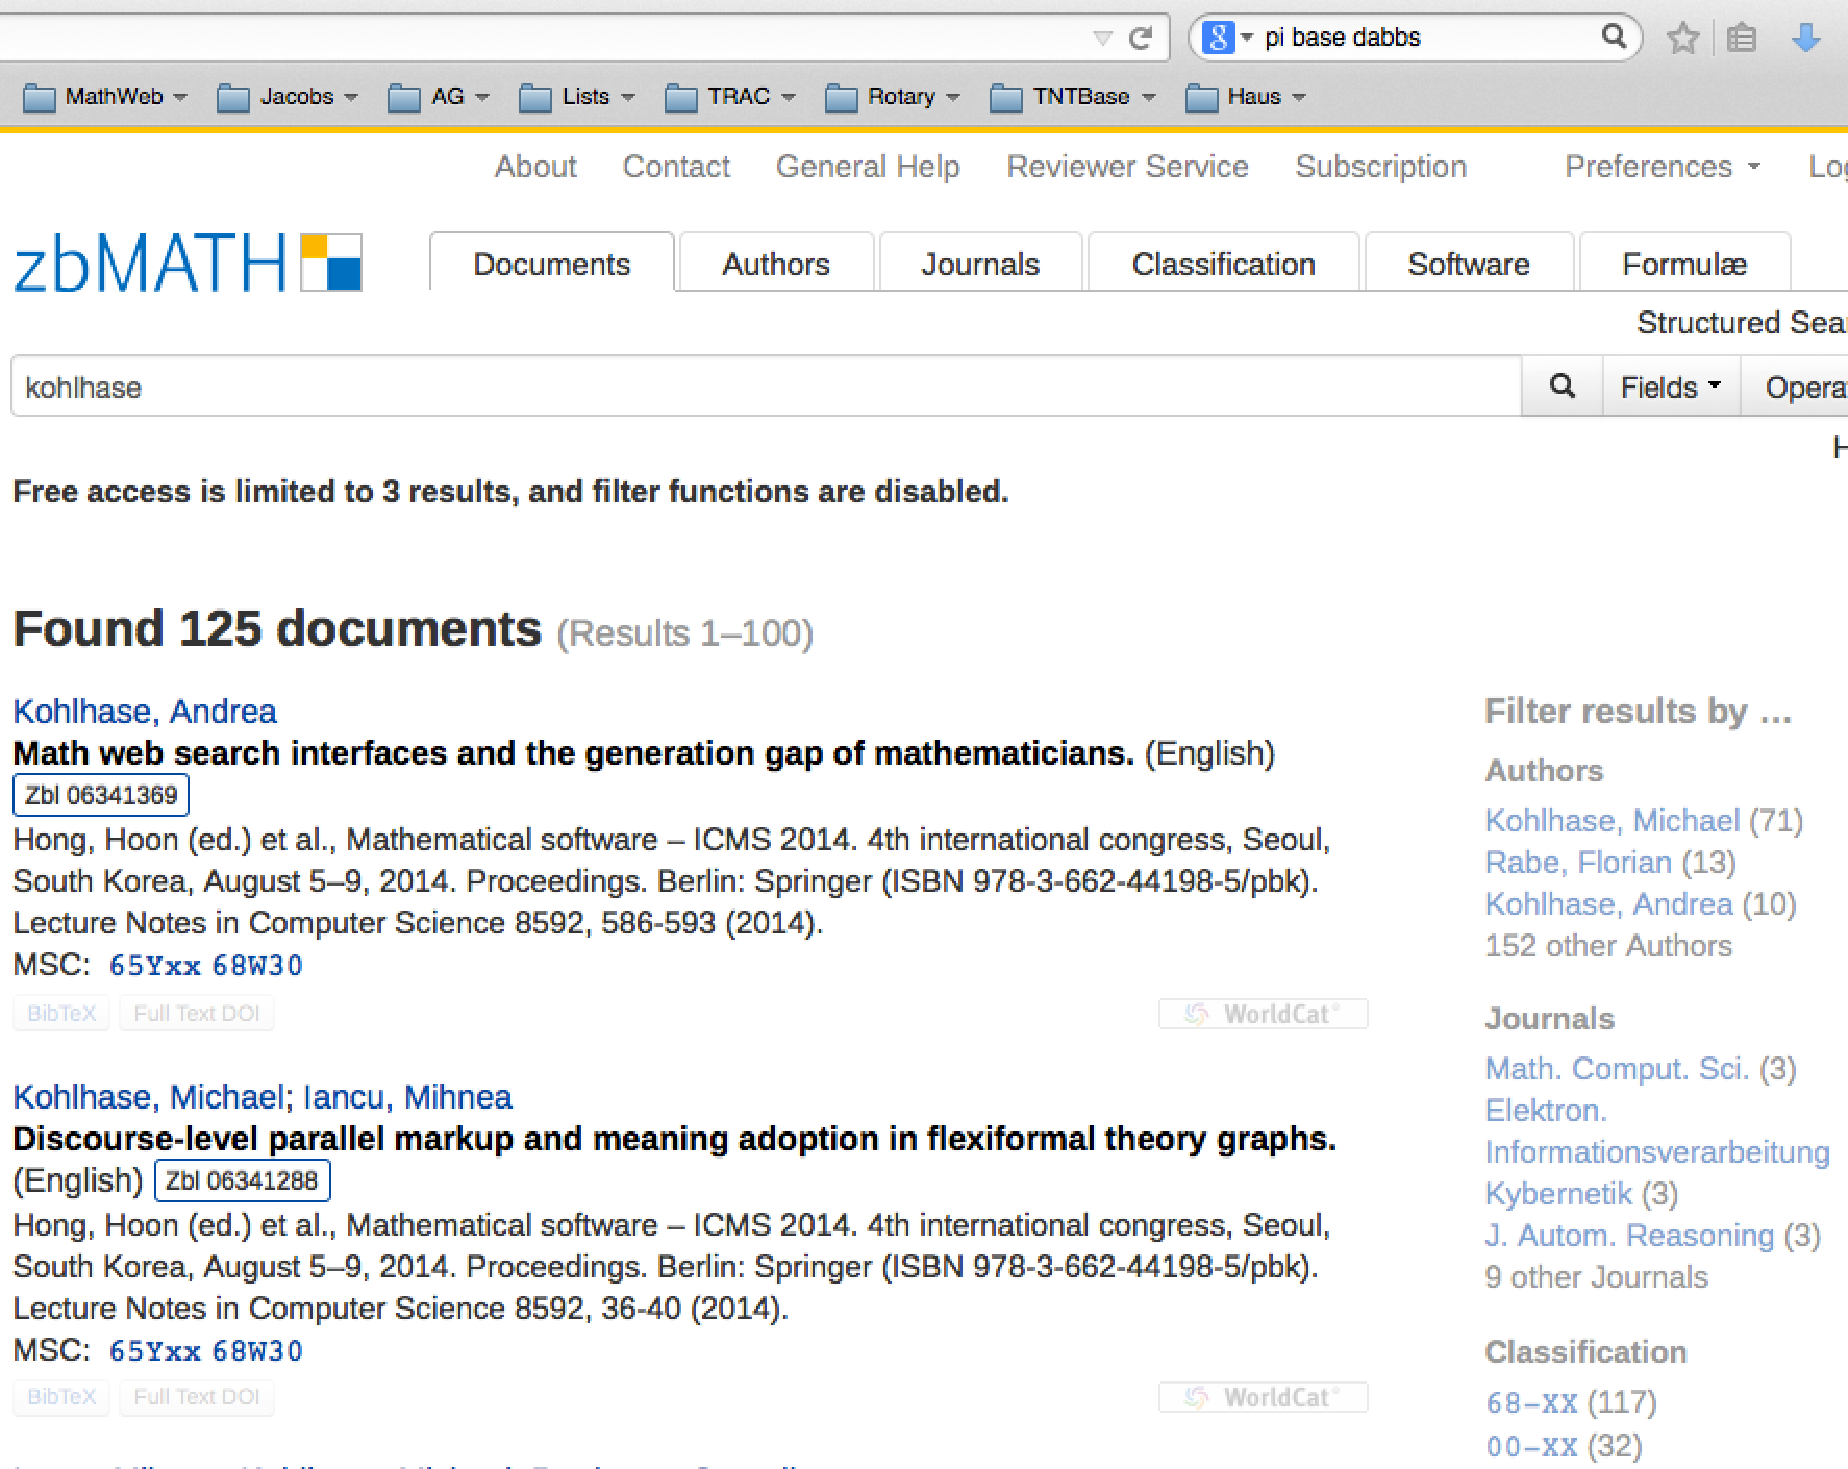
\includegraphics[width=12.7cm]{img/faceted-search.pdf}
\caption{Faceted Search in ZBMath}\label{fig:zbFaceted}
\end{figure}

There are multiple ways in which we could understand a ``math facet''.  One way
would be through the MSC classification~\cite{MSC-SKOS}.  However, this would
be rather vague because it will only provide info about the field of
mathematics to which an article belongs. If the authors use formulae from
another field in their paper, the results will suffer a drop in relevance.

We propose to solve this problem by extracting formula schemata from the query
hits as formula facets. A math facet would consist of a set of formula schemata
generated to further disambiguate the query by refining it in a new dimension.
For instance, for the query above we could have the formulae in
Figure~\ref{fig:formula-facets}, which allows the author to drill in on
\begin{inparaenum}[\em i\rm)]
\item variation theory and minimal surfaces,
\item higher-order unification, and 
\item type theory.
\end{inparaenum}
Following the \MWS (see~\ref{subsec:prelim:mws}) tradition, the red identifiers
stand for query variables, their presence making the results \textbf{formula
schemata}.

\begin{wrapfigure}r{4.6cm}\vspace*{-1em}
\begin{tabular}{l}
$\int_{\red{M}}{\red\Phi(d_p\red{f}) dvol}$\\[1ex]
$\lambda{\red{X}}.h(H^1\red{X})\cdots{H^n\red{X}}$\\[1ex]
$\frac{\red\Gamma\vdash\red{A}\gg\red\alpha}{\red{D}}$
\end{tabular}\vspace*{-.5em}
\caption{formula facets}\label{fig:formula-facets}\vspace*{-1em}
\end{wrapfigure}

These formula schemata were manually created, but for an application we need to
generate them automatically from the query. This is the algorithmic problem we
want to explore in the thesis. 


\section{Preliminaries}\label{sec:prelim}

In this section we describe the existent systems on which our work will be
based, with the intention of making this proposal self-contained. We will
present these systems in detail in the rest of this section, but
below is a summary of the role they will play in our work:
\begin{itemize}
\item \textbf{MathWebSearch} which will provide the necessary index structure
for schema search.
\item \textbf{Elasticsearch} which will provide hits in response to text query,
    as well as run aggregations on the hits.
    These hits represent formulae to be schematized.
\item \textbf{Zentralblatt Math} which will also provide formulae to be
    schematized. The algorithm to obtain these hits, corresponds to their
    current implementation of faceted search.
\end{itemize}

\subsection{MathWebSearch}\label{subsec:prelim:mws}

At its core, the \mws system (MWS) is a content-based search engine for
mathematical formulae. It indexes MathML formulae, using a technique derived
from automated theorem proving: Substitution Tree Indexing.
Recently, it was augumented with full-text search capabilities, combining
keywords query with unification-based formula search. The engine serving 
text queries is \els~\ref{subsec:prelim:els}.
From now on, in order to avoid confusion, we will refer to the core system
(providing just formula query capability) as \MWS and to the complete service
(\MWS + \els) as \tms.

The overall workflow of \tms is the following:
\begin{enumerate}
    \item HTML5 documents representing mathematical articles are
        crawled to generate \MWS harvests~\cite{mwsharvest:online}.
        \textsf{.harvest} is an extension of \mathml which \MWS can index. Its
        role is to separate the math from the text in a given document. 
    \item \MWS indexes the harvests. 
    \item a second pass is made over the harvests to generate annotated
        documents (see below). 
    \item \els indexes the annotated documents.
    \item Everything is now ready for answering queries. When a query is
        issued, \MWS will answer the mathematical part and \els will answer the
        text part.  The results will be combined through a
        NodeJS~\cite{nodejs:online} proxy to send a final result set.
\end{enumerate}

Each mathematical expression is encoded as a set of substitutions based
on a depth-first traversal of its \cmml tree.
Furthermore, each tag from the \cmml tree is encoded as a \textsf{TokenID},
to lower the size of the resulting index. The (bijective) mapping is also
stored together with the index and is needed to reconstruct the original
formula. The index itself is an in-memory trie of substitution paths.

For fast retrieval, in the leaves of the substitution tree, \MWS stores
\textsf{FormulaID}s. These are numbers uniquely associated with formulae,
and they are also used to store context and occurences about the respective
formula. They are stored in a separate LevelDB~\cite{leveldb:online} database.

A simplified sketch of the index is shown in Figure~\ref{fig:algoindex}.

\mws exposes a RESTful HTTP API which accepts \xml queries.
A valid query must obey the \cmml format, potentially augmented with
\emph{qvar} variables which match any subterms.  A \emph{qvar} variable acts as
a wildcard in a query, with the restriction that if two \emph{qvar}s have the
same name, they must be substituted in the same way.

\tms is using both \mws and \els to answer queries.
In order to achieve cooperation between the two systems, annotated documents
are used. These annotated documents contain metadata from the original document
(e.g. URI, title, author, etc.) and a list of \textsf{FormulaID}s that can be
found in that document.

\subsection{Elasticsearch}\label{subsec:prelim:els}
Elasticsearch~\cite{esl:online} is a powerful and efficient full text search
and analytics engine, built on top of Lucene. It can scale massively, because
it partitions data in shards and is also fault tolerant, because it replicates
data.  It indexes schema-free JSON documents and the search engine exposes a
RESTful web interface.  The query is also structured as JSON and supports a
multitude of features via its domain specific language:  nested queries,
filters, ranking, scoring, searching using wildcards/ranges and faceted search. 

The faceted search feature\footnote{Faceted search as such is now deprecated in
ES and was replaced by the more powerful ``aggregations''.} is of particular
interest to us.
One way to use this feature is the terms aggregation: a multi-bucket
aggregation, with dynamically built buckets.
We can specifiy an array field from a document and ask ES to count how many
unique items from the array are there in the whole index.
This list can also be sorted, e.g. most frequently occuring items first.
Additionally, we can also impose a limit on the number of the buckets (items)
for which we want to receive the count.

An ES query which would return the most frequently used formulae (and
subformulae) for ``Pierre Fermat'', is presented in Listing~\ref{lst:es_agg_query}.
The key part is the \emph{aggs} fields. We are specifying that we want an
aggregation called \textit{Formulae} on ``terms'' (i.e. we want bucket
counting) and the target of the aggregation is the fields \emph{ids}.

\begin{lstlisting}[language=json,firstnumber=1,caption=Elastic Search Term
Aggregation Query, captionpos=b, label=lst:es_agg_query]
{
  "query" : {
      "match" : {
          "body" : {
              "query" : "Pierre Fermat",
              "operator" : "and"
          }
      }
  },
  "aggs" : {
      "formulae" : {
          "terms" : { "field" : "ids" }
      }
  }
}
\end{lstlisting}

A possible response to the above query can be found in
Listing~\ref{lst:es_agg_resp}. In the response we can see the returned
aggregations. In our example there is only one and it is called
\emph{formulae}. We can find the actual result in the \emph{buckets} field. The
\textsf{key} field in the bucket corresponds to a \textsf{FormulaID}.
Here, the most frequent formulae were the one with ID 230 and the one with ID
93. The former appeared in 10 documents and the latter appeared in 9 documents.

\begin{lstlisting}[language=json,firstnumber=1,caption=Elastic Search Term
Aggregation Response, captionpos=b, label=lst:es_agg_resp]
{
    ...
    "aggregations" : {
        "formulae" : {
            "buckets" : [ 
                {
                    "key" : "230",
                    "doc_count" : 10
                },
                {
                    "key" : "93",
                    "doc_count" : 9
                },
                ...
            ]
        }
    }
}
\end{lstlisting}

\subsection{Zentralblatt Math}\label{subsec:zblatt}
\textsf{zbMATH} stores over 3 million entries corresponding to reviews or
abstracts of mathematical documents, dating back to 1826 and drawn from more
than 3,000 journals and 170,000 books\cite{zbmathabout:online}.

Among the services it provides, there is the ``structured search''.
This is essentially a faceted search engine on the textual level.
If we succeed in implementing it, we would like to integrate the 
Formula Schemata Generation Service with the zbMATH faceted search.

After running the current zbMATH faceted search implementation, a set of URIs
(referencing scientific articles which answer the user's query) will be
provided.  We should answer back with a set of formula schemata to be displayed
to the user as another facet of the result.

\subsection{arXiv}\label{subsec:arxiv}
\textbf{arXiv} is a repository of over one million publicly accessible
scientific papers in STEM fields. For the NTCIR-11
challenge~\cite{HamKohPro:man14},
MWS indexed over 8.3 million paragraphs (totaling 176 GB) from arXiv. We will
base our queries on this large index, because it provides a rich database of
highly relevant formulae. Moreover, Elasticsearch will have more formulae on
which it can run aggregations, also leading to more relevant results.


\section{The idea}\label{sec:idea}

This research project aims to develop a viable service for formulae schemata
generation and to integrate it with existing services, ultimately providing
formula faceted search. To the best of our knowledge, this problem has not been
addressed before. In this section, I propose a possible solution for math
faceted search.

\subsection{Formalizing the problem}\label{subsec:formal_problem}
Let us now formulate the problem at hand more carefully.

\begin{definition}
  Given a set $\cD$ of documents (fragments) -- e.g. generated by a search
  query, a \textbf{coverage} $0<r\leq1$, and a \textbf{width} $n$, the
  \textbf{Formula Schemata Generation} (FSG) problem requires generating
  a set $\cF$ of at most $n$ formula schemata (content MathML expressions with
  \lstinline|qvar| elements for query variables), such that $\cF$ covers $\cD$.
\end{definition}


\begin{definition}
  We say that a set $\cF$ of formula schemata \textbf{covers} a set $\cD$ of
  document fragments, with \textbf{coverage} $r$, iff at least $r \cdot |\cD|$
  formulae from $\cD$ are an instance $\sigma(f)$ of some $f\in\cF$ for a
  substitution $\sigma$.
\end{definition}

\subsection{An Algorithm for FSG}\label{subsec:fsgAlgorithm}
The FSG algorithm we propose requires a \MWS index of the corpus.
Given such an index, and a set $\cD$ of formulae (as CMML expressions), 
we can find the set $\cF$ in the following way:
\begin{itemize}
    \item Parse the given CMML expressions similarly to \MWS queries,
        to obtain their encoded DFS representations.
    \item Choose a reasonable cutoff heuristic, see~\ref{subsec:cutoffheur}.
    \item Unify each expression with the index, up to a given threshold (given by
        the above heuristic).
    \item Keep a counter for every index path associated with the unifications. 
        Since we only match up to a threshold, some formulae will be associated
        with the same path (excluding the leaves).
        We increase the counter each time we find a path already associated
        with a counter.
    \item We sort these path-counter pairs by counter in descending order and 
        take the first $n$ ($n$ being the width required by the FSG).
    \item If the threshold depth was smaller than a formula's expression
        depth, the path associated with it will have missing components. We
        replace the missing components with \lstinline|qvar|s to generate the
        schema and return the result set.
\end{itemize}

\begin{wrapfigure}r{5.6cm}\vspace*{-1em}
    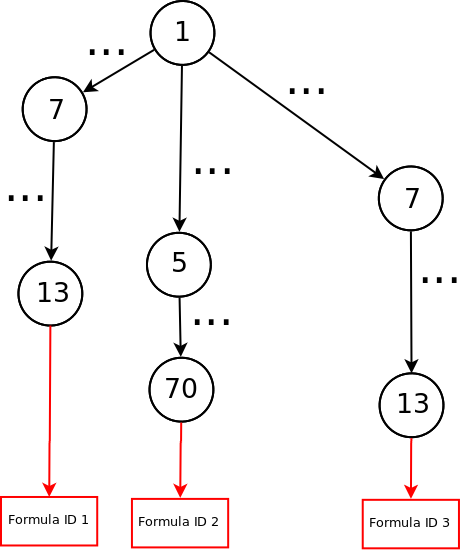
\includegraphics[scale=0.24]{img/FFG_Algo_diag.png}
\caption{Simplified index at depth 1}\label{fig:algoindex}
\end{wrapfigure}

Figure~\ref{fig:algoindex} shows a simplified \MWS index at depth 1.
The formulae's paths represent their DFS traversal.
Every formula can be reconstructed given its path in the index.
The circles represent index nodes and the number inside represents
the token's ID. When we reach a leaf node, we completely described a
formula. This is encoded in the leaf node by an ID, which can be used
to retrieve the formula from the database.
The length of the arrows symbolizes the depth of the omitted subterms
(for higher depths, we have longer arrows).
Notice how both formula with ID 1 and formula with ID 3 show the same
``path'' when ignoring subterms below a cutoff depth.

\subsection{Finding a cutoff heuristic}\label{subsec:cutoffheur}
In order to generate formula schemata, we must define a ``cutoff heuristic'',
which tells the program when two formulae belong to the same schemata class.
If there was no heuristic, two formulae would belong to the same class,
only if they were identical. However, we want formulae that have something in
common to be grouped together, even if they are not perfectly identical.

One reasonable cutoff heuristic would be a certain expression depth, given as a
parameter to the schema-engine.  In this way, a depth of 0 would always return
$?x$ which corresponds to the 0-unification. The algorithm above is based on
this heuristic.  Another possible choice for the cutoff would be expression
length.  This would output formulae which begin the same way.

\subsection{Integration with existing services}
The core engine will accept a set of CMML expressions and return a number of
schemata covering them.  The two applications that follow immediately are
Zentralblatt and Elasticsearch integration.  Using the features described
above, they are both capable of providing a set of hits belonging to some
textual context. This would represent the faceted search at the textual level.
From this set of hits, we need to obtain a set of CMML expressions, to feed
into our core algorithm. The mechanism used to achieve this is described in the
next section.

\section{Work Packages}\label{sec:timeline}

The work described in the previous section will be divided into the following
work packages:
\begin{description}
 \item [1. Core Schema Generation Algorithm] \hfill \\
     The presented core algorithm will be implemented and integrated into \mws.
 \item [2. Elasticsearch Integration] \hfill \\
     The Elasticsearch aggregation option will provide the hits as
     \textsf{FormulaID}s. These IDs represent database IDs used internally by
     \MWS to uniquely identify formulae. After receiving this set of hits, we
     can issue another query to \els to retrieve the corresponding CMML
     expressions (because the mapping from identifiers to \cmml is also stored
     in the annotated documents).

     The \els querying mechanism will be adapted to be able to handle
     aggregations. An intermediary proxy will be required to send top hits from
     \textsf{ES} to \MWS.
 \item [3. Faceted Search Frontend] \hfill \\
     A frontend will be developed to facilitate communication between users
     and the schema-search proxy mentioned above, and also to display results
     back to the user.
 \item [4. Zentralblatt Integration]\hfill \\
     Zentralblatt's structured search engine will provide the hits as documents'
     URI. We parse these documents and extract all \textsf{<expr>} nodes. We could
     also run a filter to ensure they appear only once in the resulting set, but we
     will not do it for the following reason: if a formula is included multiple
     times, the associated path through the index (using the algorithm described in
     Section~\ref{subsec:fsgAlgorithm}) will have a higher hitcount. This is
     desirable, because the formula occurred multiple times, so it is more
     representative for the set of documents.

     The schema-proxy will be upgraded, to allow Zentralblatt queries,
     with document URIs.
 \item [5. Thesis Writeup] \hfill \\
    The difficulties, findings and results of the research will be extracted
    into a writeup.
\end{description}

Figure~\ref{fig:timeline} presents the timeline for completing these milestones.

\begin{figure*}[!ht]

\hspace{-2cm}\begin{tikzpicture}
%draw horizontal line
\draw (0,0) -- (0,5.0)[dashed] node[midway,rotate=90, above=0.8cm]{Work
Packages};
\draw (0,0) -- (14,0) node[midway,below=0.8cm]{Weeks};

%draw vertical lines
\foreach \x in {0,1,2,...,14}
  \draw (\x cm,3pt) -- (\x cm,-3pt);
\foreach \x [evaluate=\x as \year using int(\x)] in {0,...,14}{
  \draw (\x,0) node[below=7pt]{$\year$};
  \draw (\x cm,3pt) -- (\x cm,-3pt);}

\draw[|-|] (0, 0.5) -- (6, 0.5) node[midway, above, align=center, text width=7cm]{Core Algorithm};
\draw[|-|] (6, 1.5) -- (8, 1.5) node[midway, above, align=center, text width=7cm]{ES Integration};
\draw[|-|] (8, 2.5) -- (9, 2.5) node[midway, above, align=center, text width=7cm]{Faceted Search Frontend};
\draw[|-|] (9, 3.5) -- (11, 3.5) node[midway, above, align=center, text width=7cm]{Zentralblatt Integration};
\draw[|-|] (9, 4.5) -- (14, 4.5) node[midway, above, align=center, text width=7cm]{Thesis Writeup};
\end{tikzpicture}

\caption{\small{Timeline}}\label{fig:timeline}
\end{figure*}

\FloatBarrier

\printbibliography

\end{document}

